
\noindent 4. Considere o seguinte algoritmo que determina o segundo maior elemento de um vetor $v[1..n]$ com $n>=2$ números positivos distintos.\\[6pt]
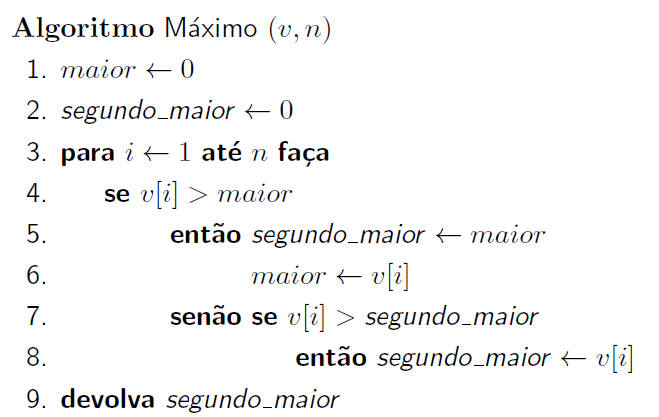
\includegraphics[width=0.6\textwidth]{algo3-4.png}

Suponha que a entrada do algoritmo é uma permutação de 1 a $n$ escolhida uniformemente dentre todas as permutaçõees de 1 a $n$.
Qual é o número esperado de comparações executadas na linha 6 do algoritmo? Qual é o número esperado de atribuições efetuadas na linha 7 do algoritmo?

Vamos calcular $E[X]$ para o algoritmo dado. Seja:\\
A = número de vezes que a linha 5 do algoritmo foi executada\\
B = número de vezes que a linha 8 do algoritmo foi executada\\

X = A + B

\begin{eqnarray*}
X_i = \left\{ \begin{array}{rl} 
 1, &\mbox{ se A ou B} \\
 0, &\mbox{ c.c}
       \end{array} \right.
\end{eqnarray*}

Logo:\\
$E[X_i] = 0 * Pr\{X_i = 0\} + 1 * Pr\{X_i = 1\} = Pr\{X_i = 1\}$\\

Sabemos que a execução da linha 8 depende da avaliação da linha 5, logo:\\
$E[X_i] = Pr\{A\} + (1 - Pr\{A\})*Pr\{B|\bar{A}\}$\\

Como já vimos para a versão original do algoritmo $\proc{Máximo}$ é $Pr\{A\} = \dfrac{1}{i}$.\\
Para a probabilidade de execução da linha 8, temos que:\\
$Pr\{B|\bar{A}\} = \dfrac{1}{1 - i}$\\

Portanto:
\begin{align*}
E[X_i] &= \bgfrac{1}{i} + \bigg(1 - \dfrac{1}{i}\bigg)\bigg(\dfrac{1}{i - 1}\bigg) \\
&= \bgfrac{1}{i} + \bigg(\dfrac{i - 1}{i}\bigg)\bigg(\dfrac{1}{i - 1}\bigg) \\
&= \dfrac{2}{i}
\end{align*}

É fato que a linha 5 sempre será executada na primeira iteração, assumindo que $v[1..n]$ contenha apenas inteiros positivos e $n >= 2$. Logo:
\begin{align*}
E[X_i] &= 1 + \sum_{i=2}^{n} \dfrac{2}{i} = 1 + 2\sum_{i=2}^{n} \dfrac{1}{i}
\end{align*}